\documentclass{beamer}
\usepackage{amsmath}
\usepackage{graphicx}
\usepackage{booktabs}

\title{Non-dimensionalizing your parameters}
\author{Laura Miller and Gemini Advanced}
\date{\today}

\begin{document}

\frame{\titlepage}

\begin{frame}
\frametitle{Non-dimensionalizing your parameters}
Why non-dimensionalize?
\begin{itemize}
\item You either need to work in real units (real size of a jellyfish, insect, etc.) or you need to report dimensionless values.
\item In the outline that follows, U’ will denote dimensionless U, and so on.
\end{itemize}.
\end{frame}

\begin{frame}
\frametitle{Characteristic length and velocity}
\begin{itemize}
\item Let U be the characteristic velocity, and L be the characteristic length
\item It is easiest to set your jellyfish bell diameter, insect wing chord, or fin chord as the characteristic length.
\item Then the domain will be bigger, of size 10L or so.
\end{itemize}
\end{frame}

\begin{frame}
\frametitle{Non-dimensional Navier-Stokes}
\begin{equation*}
\frac{\partial \mathbf{u}'}{\partial t'} + \mathbf{u}' \cdot \nabla' \mathbf{u}' = -\nabla' p' + \frac{1}{Re} \nabla'^2 \mathbf{u}'
\end{equation*}

\begin{equation*}
Re = \frac{\rho L U}{\mu}
\end{equation*}

The Navier-Stokes equation can be put into dimensionless form using the following definitions:

\begin{equation*}
\mathbf{x}' = \frac{\mathbf{x}}{L} \qquad p' = \frac{p}{\rho U^2}
\end{equation*}

\begin{equation*}
\mathbf{u}' = \frac{\mathbf{u}}{U} \qquad t' = t \frac{U}{L}
\end{equation*}

\begin{equation*}
\nabla' = L \nabla
\end{equation*}

\end{frame}


\begin{frame}{Reynolds number}

\begin{center} % Centers the image horizontally (optional)
  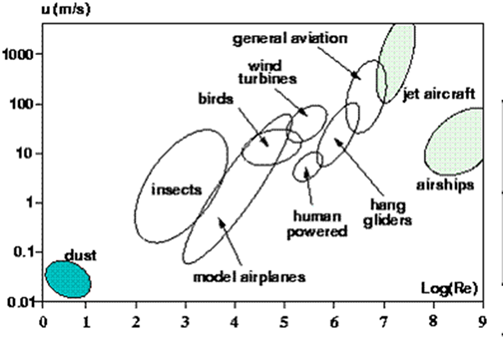
\includegraphics[width=0.85\textwidth]{../pictures/1-0/Re.png} 
  %\includegraphics[width=0.5\textwidth, height=0.4\textheight, keepaspectratio]{your_image_file.png} %Example with height and keepaspectratio
\end{center}


\end{frame}

\begin{frame}
\frametitle{Dimensionless Time and Frequency}
\begin{itemize}
\item Dimensionless time
\begin{equation*}
t’=t*U/L
\end{equation*}
\item Dimensionless frequency
\begin{equation*}
f’ = f*L/U
\end{equation*}

\item Be sure to match dimensionless time or frequency for pumping applications.
\end{itemize}
\end{frame}

\begin{frame}
\frametitle{Dimensionless Force per Unit Length}
\begin{itemize}
\item You might apply a force to a 1D fiber before it is spread to the fluid.
\item This gives you a force per unit length. To nondimensionalize it, do the following:
\item For $Re>1$
\begin{equation*}
F’=F/(\rho*L*U^2)
\end{equation*}
\item For $Re<1$
\begin{equation*}
F’=F/(\mu*U)
\end{equation*}
\end{itemize}
\end{frame}

\begin{frame}
\frametitle{What is the beam stiffness?}
\begin{itemize}
\item This is equivalent to the flexural rigidity, $EI$.
\item The flexural rigidity in 3D has units $N*m^2$, and is given by EI, where E is the elastic or Young’s modulus ($N/m^2$) and I is the second moment of area (in units of $length^4$).
\item The flexural rigidity in 2D has units N*m.
\end{itemize}
\end{frame}

\begin{frame}
\frametitle{Approximate Young’s modulus for various materials}

\tiny
\setlength\tabcolsep{2pt} % Reduce column spacing
\begin{tabular}{lrrr}
\toprule
Material & \multicolumn{2}{c}{Approximate Young's modulus} \\
\cmidrule(r){2-3} & GPa & lbf/in$^2$ (psi) \\
\midrule
Rubber (small strain) & 0.01–0.1 & 1,450–14,503 \\
Low density polyethylene & 0.11–0.45 & 16,000–65,000 \\
Diatom frustules (largely silicic acid) & 0.35–2.77 & 50,000–400,000 \\
PTFE (Teflon) & 0.5 & 75,000 \\
HDPE & 0.8 & 116,000 \\
Bacteriophage capsids & 1–3 & 150,000–435,000 \\
Polypropylene & 1.5–2 & 218,000–290,000 \\
Polyethylene terephthalate (PET) & 2.2–2.7 & 290,000–390,000 \\
Nylon & 2–4 & 290,000–580,000 \\
Polystyrene & 3–3.5 & 440,000–510,000 \\
Medium-density fiberboard (MDF) & 4 & 580,000 \\
Oak wood (along grain) & 11 & 1.60 $\times$ 10$^6$ \\
Human Cortical Bone & 14 & 2.03 $\times$ 10$^6$ \\
Glass-reinforced polyester matrix & 17.2 & 2.49 $\times$ 10$^6$ \\
Aromatic peptide nanotubes & 19–27 & 2.76 $\times$ 10$^6$–3.92 $\times$ 10$^6$ \\
High-strength concrete & 30 & 4.35 $\times$ 10$^6$ \\
Carbon fiber reinforced plastic (50/50 fibre/matrix, biaxial fabric) & 30–50 & 4.35 $\times$ 10$^6$–7.25 $\times$ 10$^6$ \\
Hemp fiber & 35 & 5.08 $\times$ 10$^6$ \\
Magnesium metal (Mg) & 45 & 6.53 $\times$ 10$^6$ \\
Glass (see chart) & 50–90 & 7.25 $\times$ 10$^5$ - 13.1 $\times$ 10$^6$ \\
Flax fiber & 58 & 8.41 $\times$ 10$^6$ \\
Aluminum & 69 & 10.0 $\times$ 10$^6$ \\
Mother-of-pearl (nacre, largely calcium carbonate) & 70 & 10.2 $\times$ 10$^6$ \\
Aramid & 70.5–112.4 & 10.2 $\times$ 10$^6$ - 16.3 $\times$ 10$^6$ \\
Tooth enamel (largely calcium phosphate) & 83 & 12.0 $\times$ 10$^6$ \\
\bottomrule
\end{tabular}

\end{frame}


\begin{frame}{Second moment of area}
\textbf{Definition}

The second moment of area for an arbitrary shape with respect to an arbitrary axis \( BB \) is defined as

\[
J_{BB} = \int_A \rho^2 \, dA
\]

\( dA \) = Differential area of the arbitrary shape

\( \rho \) = Distance from the axis \( BB \) to \( dA \)

For example, when the desired reference axis is the x-axis the second moment of area, \( I_{xx} \) (often denoted as \( I_x \)) can be computed in Cartesian coordinates as

\[
I_x = \int_A \int y^2 \, dx \, dy
\]
\end{frame}

\begin{frame}{Rectangle with centroid at the origin}
\\
\\
Consider a rectangle with base \( b \) and height \( h \) whose centroid is located at the origin. \( I_x \) represents the second moment of area with respect to the x-axis; \( I_y \) represents the second moment of area with respect to the y-axis; \( J_z \) represents the polar moment of inertia with respect to the z-axis.
\tiny % Make the whole frame smaller
\[
I_x = \int_A y^2 \, dA = \int_{-b/2}^{b/2} \int_{-h/2}^{h/2} y^2 \, dy \, dx = \frac{1}{3} \int_{-b/2}^{b/2} \frac{h^3}{4} \, dx = \frac{bh^3}{12}
\]

\[
I_y = \int_A x^2 \, dA = \int_{-b/2}^{b/2} \int_{-h/2}^{h/2} x^2 \, dx \, dy = h \int_{-b/2}^{b/2} x^2 \, dx = \frac{b^3h}{12}
\]

\[
J_z = I_x + I_y = \frac{bh^3}{12} + \frac{b^3h}{12} = \frac{bh}{12} (b^2 + h^2) \quad \text{(see Perpendicular axis theorem)}
\]

% Place holder for the image of the rectangle
\begin{center}
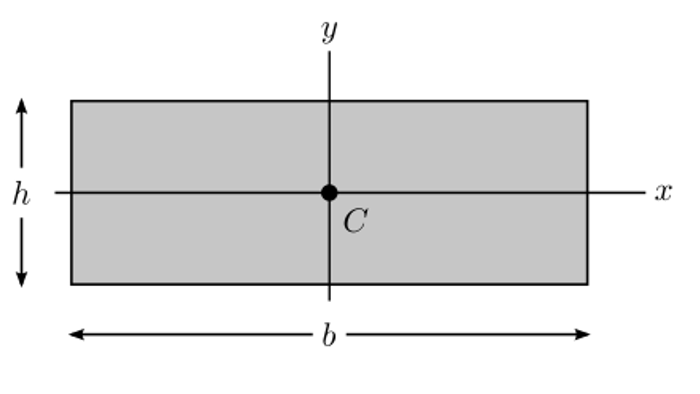
\includegraphics[width=0.4\textwidth]{../pictures/1-0/IJ.png} % Slightly smaller image
\end{center}
\end{frame}

\begin{frame}{Dimensionless Bending Coefficient in 2D}
\begin{itemize}
\item Note that below \( k_{beam} \) in 2D is assumed to have units of \( N \cdot m \).

\item In 2D, the relationship for \( Re > 1 \) is:
\[
k'_{beam} = \frac{k_{beam}}{\rho U^2 L^3}
\]

\item In 2D, the relationship for \( Re < 1 \) is:
\[
k'_{beam} = \frac{k_{beam}}{\mu U L^2}
\]
\end{itemize}
\end{frame}

\begin{frame}{Dimensionless Stretching Coefficient}
\begin{itemize}
\item Note that below \( k_{spring} \) is assumed to have units of \( N/m \).
\item In 2D, the relationship for \( Re > 1 \) is:
\[
k'_{spring} = \frac{k_{spring}}{\rho U^2 L}
\]

\item In 2D, the relationship for \( Re < 1 \) is:
\[
k'_{spring} = \frac{k_{spring}}{\mu U}
\]
\end{itemize}
\end{frame}

\begin{frame}{Viscosity}
\begin{itemize}
\item Often we change $Re$ by changing the dynamic viscosity, $\mu$.
\item Rather than nondimensionalizing the dynamic or kinematic viscosity, you can just report the \( Re \) (since you have already defined \( U \) and \( L \)).
\end{itemize}
\end{frame}

\begin{frame}{Estimate \( k_{beam} \)}
\begin{itemize}
\item By using the dimensionless beam stiffness \( k'_{beam} \), one can make an educated guess for \( k_{beam} \).

\item Setting \( k'_{beam} = 10 \) typically results in a little bit of bending (maybe 2 - 10 degrees).

\item In 2D, the relationship for \( Re > 1 \) is:
\[
k'_{beam} = \frac{k_{beam}}{\rho U^2 L^3}
\]
\( U \) is the characteristic velocity (try \( U_{max} \)) and \( L \) is the characteristic length. I would use the length of the boundary.

\item Warning to user: these are really rough estimates.
\end{itemize}
\end{frame}

\begin{frame}{Estimate \( k_{spring} \)}
\begin{itemize}
\item By estimating the force acting on the boundary (\( F_b \)) and the desired displacement (\( x_s \)), one can make an educated guess for \( k_{spring} \).

\item The idea is to set \( k_{spring} = \frac{F_b}{x_s} \).

\item Choose \( x_s \) to be the maximum desired displacement from the target point or the maximum amount of displacement from a resting length.

\item The estimate for \( F_b \) will depend on \( Re \) and dimension (\( dim \)). For the characteristic velocity, \( U \), I recommend using \( U_{max} \).
\[
F_b \sim \frac{1}{2} \rho \, dx^{(dim-1)} U^2 \quad \text{for } Re > 1
\]
\[
F_b \sim \mu \, dx \, U \quad \text{for } Re < 1
\]

\item Warning to user: these are really rough estimates.
\end{itemize}
\end{frame}

\begin{frame}{Estimate Damping}
\begin{itemize}
\item The goal is to make the springs close to critically damped: \url{http://en.wikipedia.org/wiki/Damping}

\item This means setting the damping coefficient, \( c = 2 \sqrt{k_{spring} m} \).

\item The hard part is estimating \( m \). Recall the boundary is massless, but there is the added mass of the fluid.

\item My recommendation is to try setting \( m = \rho (dx^{dim}) \).

\item Warning to user: these are really rough estimates.
\end{itemize}
\end{frame}

\begin{frame}{Strouhal number}
\small
\textit{From Wikipedia, the free encyclopedia}

\medskip

In dimensional analysis, the \textbf{Strouhal number} (St) is a \textbf{dimensionless number} describing oscillating flow mechanisms. The parameter is named after Vincenc Strouhal, a Czech physicist who experimented in 1878 with wires experiencing \textbf{vortex shedding} and singing in the wind. The Strouhal number is an integral part of the fundamentals of fluid mechanics.

\medskip

The Strouhal number is often given as;

\begin{equation*}
\text{St} = \frac{fL}{V},
\end{equation*}

where \(f\) is the frequency of \textbf{vortex shedding}, \(L\) is the characteristic length (for example hydraulic diameter, or chord length) and \(V\) is the velocity of the fluid. In certain cases like heaving (plunging) flight, this characteristic length is the amplitude of oscillation.

\end{frame}

\begin{frame}{Strouhal number in swimming and flying}
\begin{itemize}
\item In terms of animal locomotion, $St$ describes the tail or wing kinematics of swimming and flying animals is the Strouhal number, \( St = \frac{fA}{U} \), which divides stroke frequency (\( f \)) and amplitude (\( A \)) by forward speed (\( U \)).

\item \( St \) is known to govern a well-defined series of vortex growth and shedding regimes for airfoils undergoing pitching and heaving motions.

\item Propulsive efficiency is high over a narrow range of \( St \) and usually peaks within the interval \( 0.2 < St < 0.4 \).
\end{itemize}
\end{frame}


\begin{frame}{Womersley number}
\tiny
\textit{From Wikipedia, the free encyclopedia}

\medskip

The Womersley number ($\alpha$) is a dimensionless number in biofluid mechanics. It is a dimensionless expression of the \textbf{pulsatile flow frequency} in relation to \textbf{viscous effects}. It is named after John R. Womersley (1907-1958) for his work with bloodflow in arteries. The Womersley number is important in keeping \textbf{dynamic similarity} when scaling an experiment. An example of this is scaling up the vascular system for experimental study. The Womersley number is also important in determining the thickness of the \textbf{boundary layer} to see if entrance effects can be ignored.

\medskip

\textbf{Derivation} 

\medskip

The Womersley number, usually denoted $\alpha$, is defined by the relation

\begin{equation*}
\alpha^2 = \frac{\text{transient inertial force}}{\text{viscous force}} = \frac{\rho \omega U}{\mu U L^{-2}} = \frac{\omega L^2}{\mu \rho^{-1}} = \frac{\omega L^2}{\nu},
\end{equation*}

where \(L\) is an appropriate length scale (for example the radius of a pipe), \(\omega\) is the angular frequency of the oscillations, and \(\nu\), \(\rho\), \(\mu\) are the kinematic viscosity, density, and dynamic viscosity of the fluid, respectively. The Womersley number is normally written in the powerless form

\begin{equation*}
\alpha = L \left( \frac{\omega}{\nu} \right)^{\frac{1}{2}} = L \left( \frac{\omega \rho}{\mu} \right)^{\frac{1}{2}}
\end{equation*}

It can also be written in terms of the dimensionless Reynolds number (Re) and Strouhal number (Sr):

\begin{equation*}
\alpha = (2 \pi Re \, Sr)^{1/2}.
\end{equation*}

\end{frame}

\begin{frame}{Some typical values for the Womersley number}

Some typical values for the Womersley number in the cardiovascular system for a canine at a heart rate of 2 Hz are:

\begin{itemize}
    \item Ascending Aorta — 13.2
    \item Descending Aorta — 11.5
    \item Abdominal Aorta — 8
    \item Femoral Artery — 3.5
    \item Carotid Artery — 4.4
    \item Arterioles — 0.04
    \item Capillaries — 0.005
    \item Venules — 0.035
    \item Inferior Vena Cava — 8.8
    \item Main Pulmonary Artery — 15
\end{itemize}

\end{frame}

\begin{frame}{The Péclet number (Pe)}

The Péclet number (Pe) is a class of \textbf{dimensionless numbers} relevant in the study of transport phenomena in a continuum. It is named after the French physicist Jean Claude Eugène Péclet. It is defined to be the ratio of the rate of \textbf{advection} of a physical quantity by the flow to the rate of \textbf{diffusion} of the same quantity driven by an appropriate gradient. In the context of \textbf{mass transfer}, the Péclet number is the product of the Reynolds number and the Schmidt number. In the context of the \textbf{thermal fluids}, the thermal Peclet number is equivalent to the product of the Reynolds number and the Prandtl number.

\medskip

The Péclet number is defined as:

\begin{equation*}
\text{Pe} = \frac{\text{advective transport rate}}{\text{diffusive transport rate}}
\end{equation*}

\medskip

For mass transfer, it is defined as:

\begin{equation*}
\text{Pe}_L = \frac{Lu}{D} = \text{Re}_L \, \text{Sc}
\end{equation*}

\end{frame}

\begin{frame}{Efficiency - a highly controversial topic!}
Thermodynamic efficiency: the ratio of the work done by something to the energy supplied to it.

The ratio between the useful output of a device and the input, in energy terms.

What is useful output in terms of energy?
\begin{itemize}
    \item Kinetic energy - \( \frac{1}{2} mv^2 \) (units of \( kg \cdot m^2/s^2 = N \cdot m \))
    \item Potential energy - \( mass \cdot g \cdot h \) (units of \( kg \cdot (m/s^2) \cdot m = N \cdot m \))
\end{itemize}
Formally, useful work is changing kinetic or potential energy by accelerating or changing height, respectively.

No useful work is done in steady state swimming!

Do all steady state swimmers have zero efficiency?

Need to carefully define another metric (performance metric).
\end{frame}


\begin{frame}{Cost of Transport}
\( COT \) = Power expenditure per unit length traveled.

Recall the following relationships:
\begin{itemize}
    \item work = force \( \cdot \) distance (units \( N \cdot m \))
    \item power = work / time = force \( \cdot \) velocity (units \( N \cdot m/s \))
\end{itemize}
You can calculate this by estimating the force input at each time step multiplied by the velocity of the boundary doing the work.
\end{frame}


\end{document}